\documentclass[10pt,twocolumn]{article}
\usepackage{geometry}
\geometry{verbose,headsep=3cm,tmargin=2.5cm,bmargin=2.5cm,lmargin=2.0cm,rmargin=2.0cm}
\usepackage{graphicx}
\usepackage{xcolor}
\usepackage[font=small]{caption}
\usepackage{amsmath,amssymb,latexsym}
\usepackage{marvosym}
\usepackage{url}
\usepackage{lipsum}
\usepackage{bm}
\usepackage{float}
\usepackage[english]{babel}
\usepackage{hyperref}
\usepackage{epsf}
\usepackage{float}
\usepackage{mathpazo}
\usepackage{pifont}
\usepackage{wrapfig}
\usepackage{multicol}
\usepackage{enumitem}
\usepackage{xcolor}
\usepackage{framed}
\usepackage[utf8]{inputenc}
% Document font:
\usepackage{charter}
\graphicspath{{GPR-Python/}{DWGs/}}

\newcommand{\highlight}[1]{%
  \colorbox{orange!50}{$\displaystyle#1$}}
% Default fixed font does not support bold face
\DeclareFixedFont{\ttb}{T1}{txtt}{bx}{n}{10} % for bold
\DeclareFixedFont{\ttm}{T1}{txtt}{m}{n}{10}  % for normal

% Custom colors
\usepackage{color}
\definecolor{deepblue}{rgb}{0,0,0.5}
\definecolor{deepred}{rgb}{0.6,0,0}
\definecolor{deepgreen}{rgb}{0,0.5,0}

\usepackage{listings}

% Python style for highlighting
\newcommand\pythonstyle{\lstset{
language=Python,
basicstyle=\ttm,
otherkeywords={self},             % Add keywords here
keywordstyle=\ttb\color{deepblue},
emph={MyClass,__init__},          % Custom highlighting
emphstyle=\ttb\color{deepred},    % Custom highlighting style
stringstyle=\color{deepgreen},
frame=tb,                         % Any extra options here
showstringspaces=false            % 
}}


% Python environment
\lstnewenvironment{python}[1][]
{
\pythonstyle
\lstset{#1}
}
{}

% Python for external files
\newcommand\pythonexternal[2][]{{
\pythonstyle
\lstinputlisting[#1]{#2}}}

% Python for inline
\newcommand\pythoninline[1]{{\pythonstyle\lstinline!#1!}}



\begin{document}

\twocolumn[{
\begin{@twocolumnfalse}

  \begin{center}
%\textcolor{lgray}
    \vskip-5em

    \hfill
    \fontsize{10}{10}\selectfont {\textit{Bruxelles, November 2018 - Salt Lake City, March 2020}}
    \vskip2ex
	\vspace{5ex}
    \fontsize{20}{10}\selectfont {Notes on Gaussian Process Regression}
      \vspace{1ex}
      
      \fontsize{16}{10}\selectfont {(with Python examples)}
  \noindent%
    
\vskip1ex

{\rule{\textwidth}{0.5pt}}

  \end{center}
  
    \fontsize{7}{10}\selectfont {This work is licensed under the Creative Commons Attribution-NonCommercial-ShareAlike 4.0 International (CC BY-NC-SA 4.0) license.}

\vspace{6mm}

\end{@twocolumnfalse}
}]

%%% HEADER END -----------------------------------------------------------
% ------------------------------------------------------------------------

\vspace{10mm}

\setlength{\parindent}{0cm}

\fontsize{14}{10}\selectfont {Kamila Zdybał}

\vspace{2mm}

\fontsize{8}{10}\selectfont {\textit{Université libre de Bruxelles, kamila.zdybal@ulb.ac.be}}

\fontsize{8}{10}\selectfont {\textit{kamilazdybal.github.io/science-docs, kamila.zdybal@gmail.com}}

\section*{Preface}

\,\,

I would like to give credit to many wonderful resources that let me study GPR with joy. In particular, a great lecture by Professor Anna Scaife \cite{Scaife} is among the ones that gave me a lot of intuition during my first encounter. Figures presented in section \ref{sec:meaning-of-hyp} are reproduction of figures from Professor Scaife's lecture. I also gained deeper mathematical understanding of GPR from the great textbook \textit{Gaussian Process for Machine Learning} by C. E. Rasmussen and C. Williams \cite{Rasmussen}. Many other resources helped me in understanding GPR and writing this short document. I listed all of them in the References.

I also acknowledge the help that I got from the Cross Validated Stack Exchange community, in particular in response to my question \cite{SE}.

\,\,

Please feel free to contact me with any suggestions, corrections or comments.

\section*{Keywords}

\textit{Gausssian Process Regression (GPR), regression, covariance function, covariance kernel}

\tableofcontents

\section{Introduction}

\textit{Gaussian Process Regression} (GPR) is a regression technique which does not restrict what functions are used to model the data - unlike linear or polynomial regression for instance. Instead, we allow many possible functions from a certain pre-specified \textit{pool}. To each of these function we attribute a certain probability of how likely we believe it will fit well our data and update this function pool as new data points are observed. This brings us to the first concept worth discussing: \textit{distribution over functions}.


%\section{World according to Bayes}



\subsection{Distribution over functions} \label{sec:dist_over_fun}

In GPR we allow many types of functions and we attribute a certain likelihood to each of them, quantifying our belief that it can well regress our data. The space of these functions is mapped on a space of likelihoods and such mapping is called a \textit{distribution over functions}. Visually, one may treat this as a probability distribution drawn "above" the space of all possible functions - some functions are more likely, some are less likely.

\begin{figure}[H]
\centering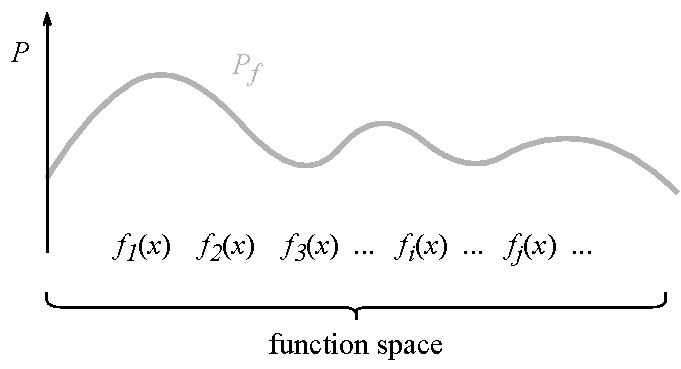
\includegraphics[width=8.5cm]{distribution-over-functions.pdf}
\caption{Conceptual visualisation of distribution over functions.}
\label{fig:distr_over_fun}
\end{figure}

\section{Probability}

\subsection{Prior and posterior}

Two words that will be often used in GP are \textit{prior} and \textit{posterior}. The prior and posterior probabilities in GP are often linked to functions and it is important to understand their notion.

The \textbf{\textit{prior probability}} is the probability we assign to a specific object (event) before we collect further evidence or make observations that can change it. It can be viewed as an "initial guess" or "initial belief" about the given system. The \textbf{\textit{posterior probability}} is the updated prior probability that takes into account the new observations or evidence. Conceptually, we may write the following:

\begin{equation}
\text{prior distribution} + \text{data} = \text{posterior distribution}
\end{equation}

As explained in section \ref{sec:dist_over_fun}, in GP we encounter probabilities associated with functions. The prior will be the functions that we believe will fit our data well before we actually attempt fitting these functions to new observation points. After the observations have been made, the functions get the probability "update" to better fit the newly arrived points and these functions that are left will become our posterior.


% \subsection{Likelihood and marginal likelihood}


\section{Covariance matrix}

Let's think about a dot product between two vectors $x_i$ and $x_j$:

\begin{equation}
\text{dot}(x_i, x_j) = |x_i| |x_j| \text{cos}(\phi)
\end{equation}

It describes the amount of projection of vector $x_i$ onto $x_j$ (and vice versa) and can be useful when we need to know how much one vector points in the direction of the other.

Now imagine that you have a data set $\mathbf{X}$ with $n$ vectors represented by the columns of this data set, and you would like to know what is the dot product of every possible pair drawn from these vectors. In other words, you would like to know how correlated are all vectors with each other. You can achieve this "global" dot product by multiplying:

\begin{equation}\label{eq:covariance-matrix}
\mathbf{S} = \mathbf{X}^T \mathbf{X} 
\end{equation}

the result $\mathbf{S}$ is called the \textit{covariance matrix}. Notice that every entry $(i,j)$ in this matrix is a dot product $\text{dot}(x_i, x_j)$ and it either represent the covariance:

\begin{equation}
\text{dot}(x_i, x_j) = \text{cov}(x_i, x_j) \,\,\, \text{for} \,\,\, i \neq j
\end{equation}

or the variance:

\begin{equation}
\text{dot}(x_i, x_j) = \text{var}(x_i, x_j) \,\,\, \text{for} \,\,\, i = j
\end{equation}

The covariance matrix is symmetric due to symmetry: $\text{dot}(x_i, x_j) = \text{dot}(x_j, x_i)$.

\section{Covariance kernels}

The \textit{covariance kernel} is essentialy a function that populates the covariance matrix. This makes our life easier, since first, this matrix might be computationally expensive to evaluate using eq.(\ref{eq:covariance-matrix}) - notice that for a given size $n \times n$ of the covariance matrix, the data set $\mathbf{X}$ can have arbitrarily many observations (columns of $\mathbf{X}$ can be arbitrarily long). Second, we can easily implement the underlying structure to the covariance.

The only restriction is that the covariance kernel has to be designed such that there is symmetry: $K(x_i, x_j) = K(x_j, x_i)$ (to assure symmetry of the covariance matrix).

% At this point you probably wonder: but when we populate the covariance matrix in this "artificial" way, will it still make any sense to us? Will it still represent the covariance-variance of our original columns of $\mathbf{X}$?

\subsection{Examples}

Squared Exponential kernel:

\begin{equation}
K(x_i, x_j) = h^2 \exp(\frac{- (x_i - x_j)^2}{\lambda^2})
\end{equation}


\subsection{The meaning of hyperparameters} \label{sec:meaning-of-hyp}

We will now take a look at the Squared Exponential kernel which was introduced before and explore how the hyperparameters affect the structure of the covariance matrix and the type of priors drawn from the distribution.

%\pythoninline{y = np.random.multivariate_normal(mean, cov)}

Let's increase the kernel width $\lambda$ first and draw the covariance matrix (the upper three figures in Fig.\ref{fig:SE-kernel-width}). As $\lambda$ increases, even the variables which are further away are correlated. That is also reflected in the type of prior that is drawn from this distrbution - three bottom figures in Fig.\ref{fig:SE-kernel-width}. For $\lambda = 5$ the prior looks much less random than for $\lambda = 0.1$ - the variable's value at any point is strongly affected by the values of the nearby variables. To put it in yet other words, the derivatives at any point change much less drastically at $\lambda = 5$ than at $\lambda = 0.1$.

\begin{figure}[H]
\centering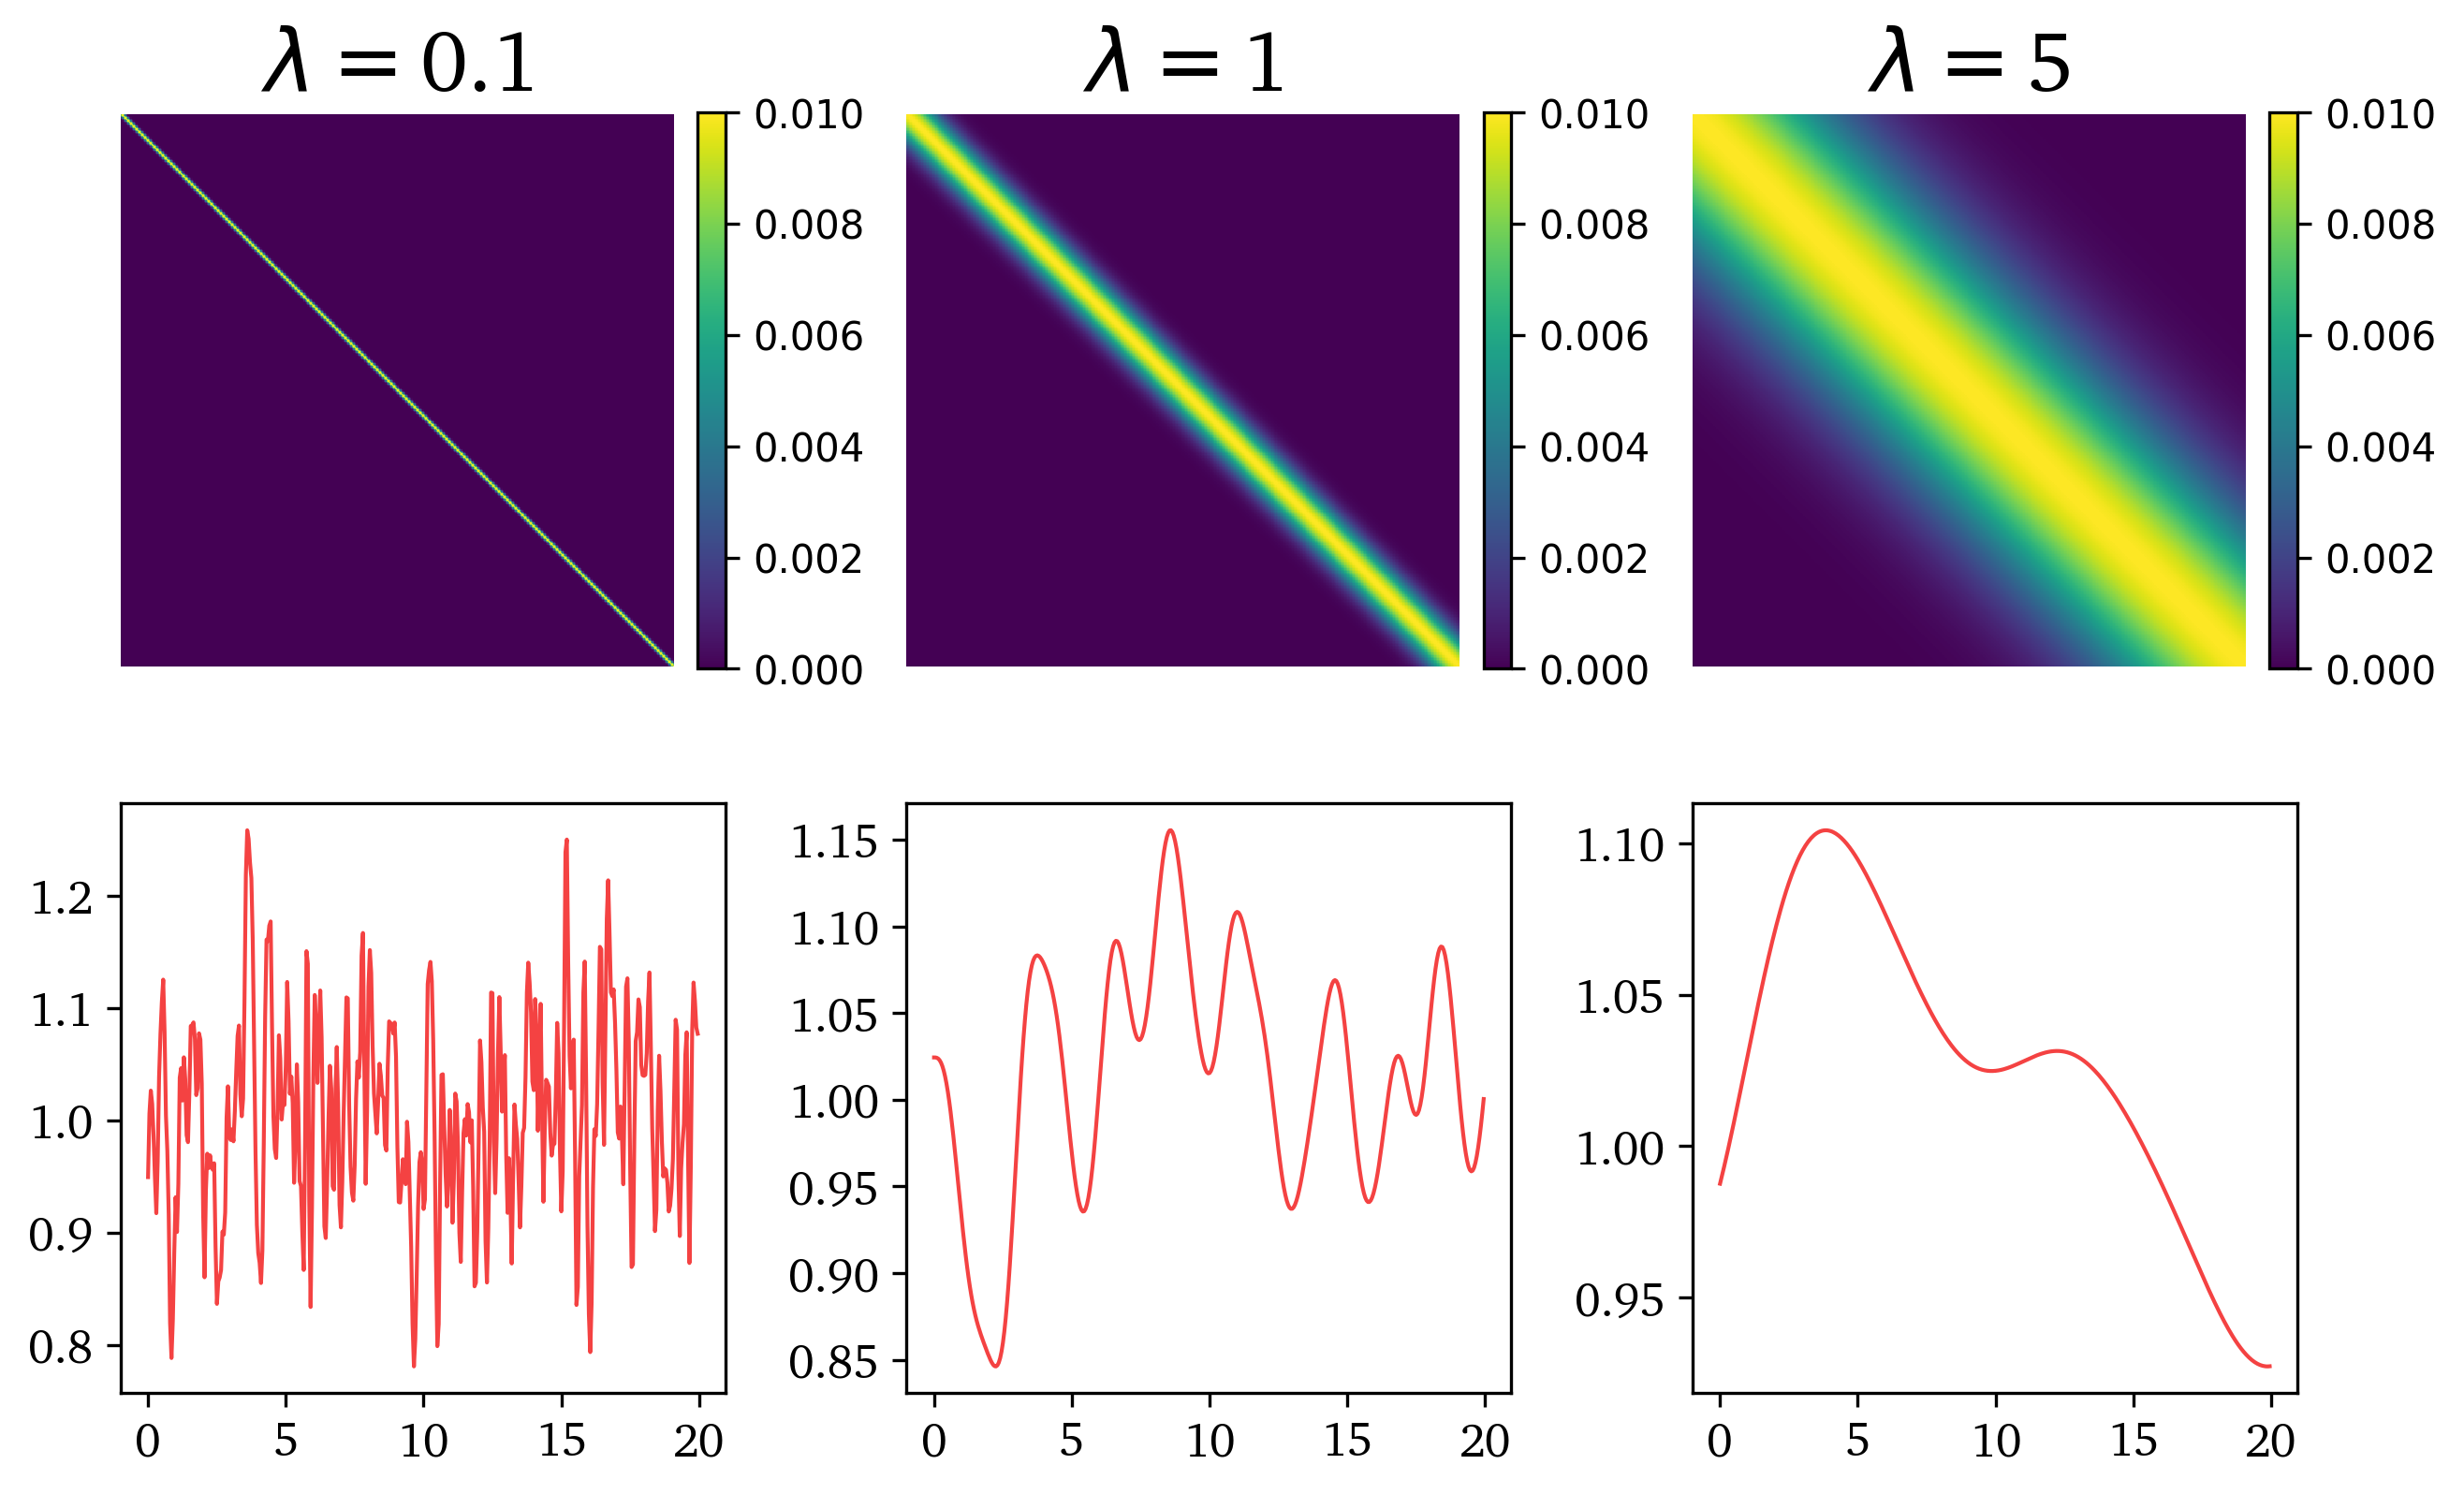
\includegraphics[width=8.5cm]{cov-Kernel-SE-changing-lambda-tex.png}
\caption{Adjusting the kernel width $\lambda$.}
\label{fig:SE-kernel-width}
\end{figure}

Varying the scaling factor $h$, the priors are now stationary and the covariance has the same width. What is changing is the numerical value of the covariance matrix. For every $h$ the covariance matrix gets scaled and the largest elements in the matrix are always equal to $h^2$. Thus, varying $h$  will vary the "strength" of the correlation of any variables that are correlated in the first place.

\begin{figure}[H]
\centering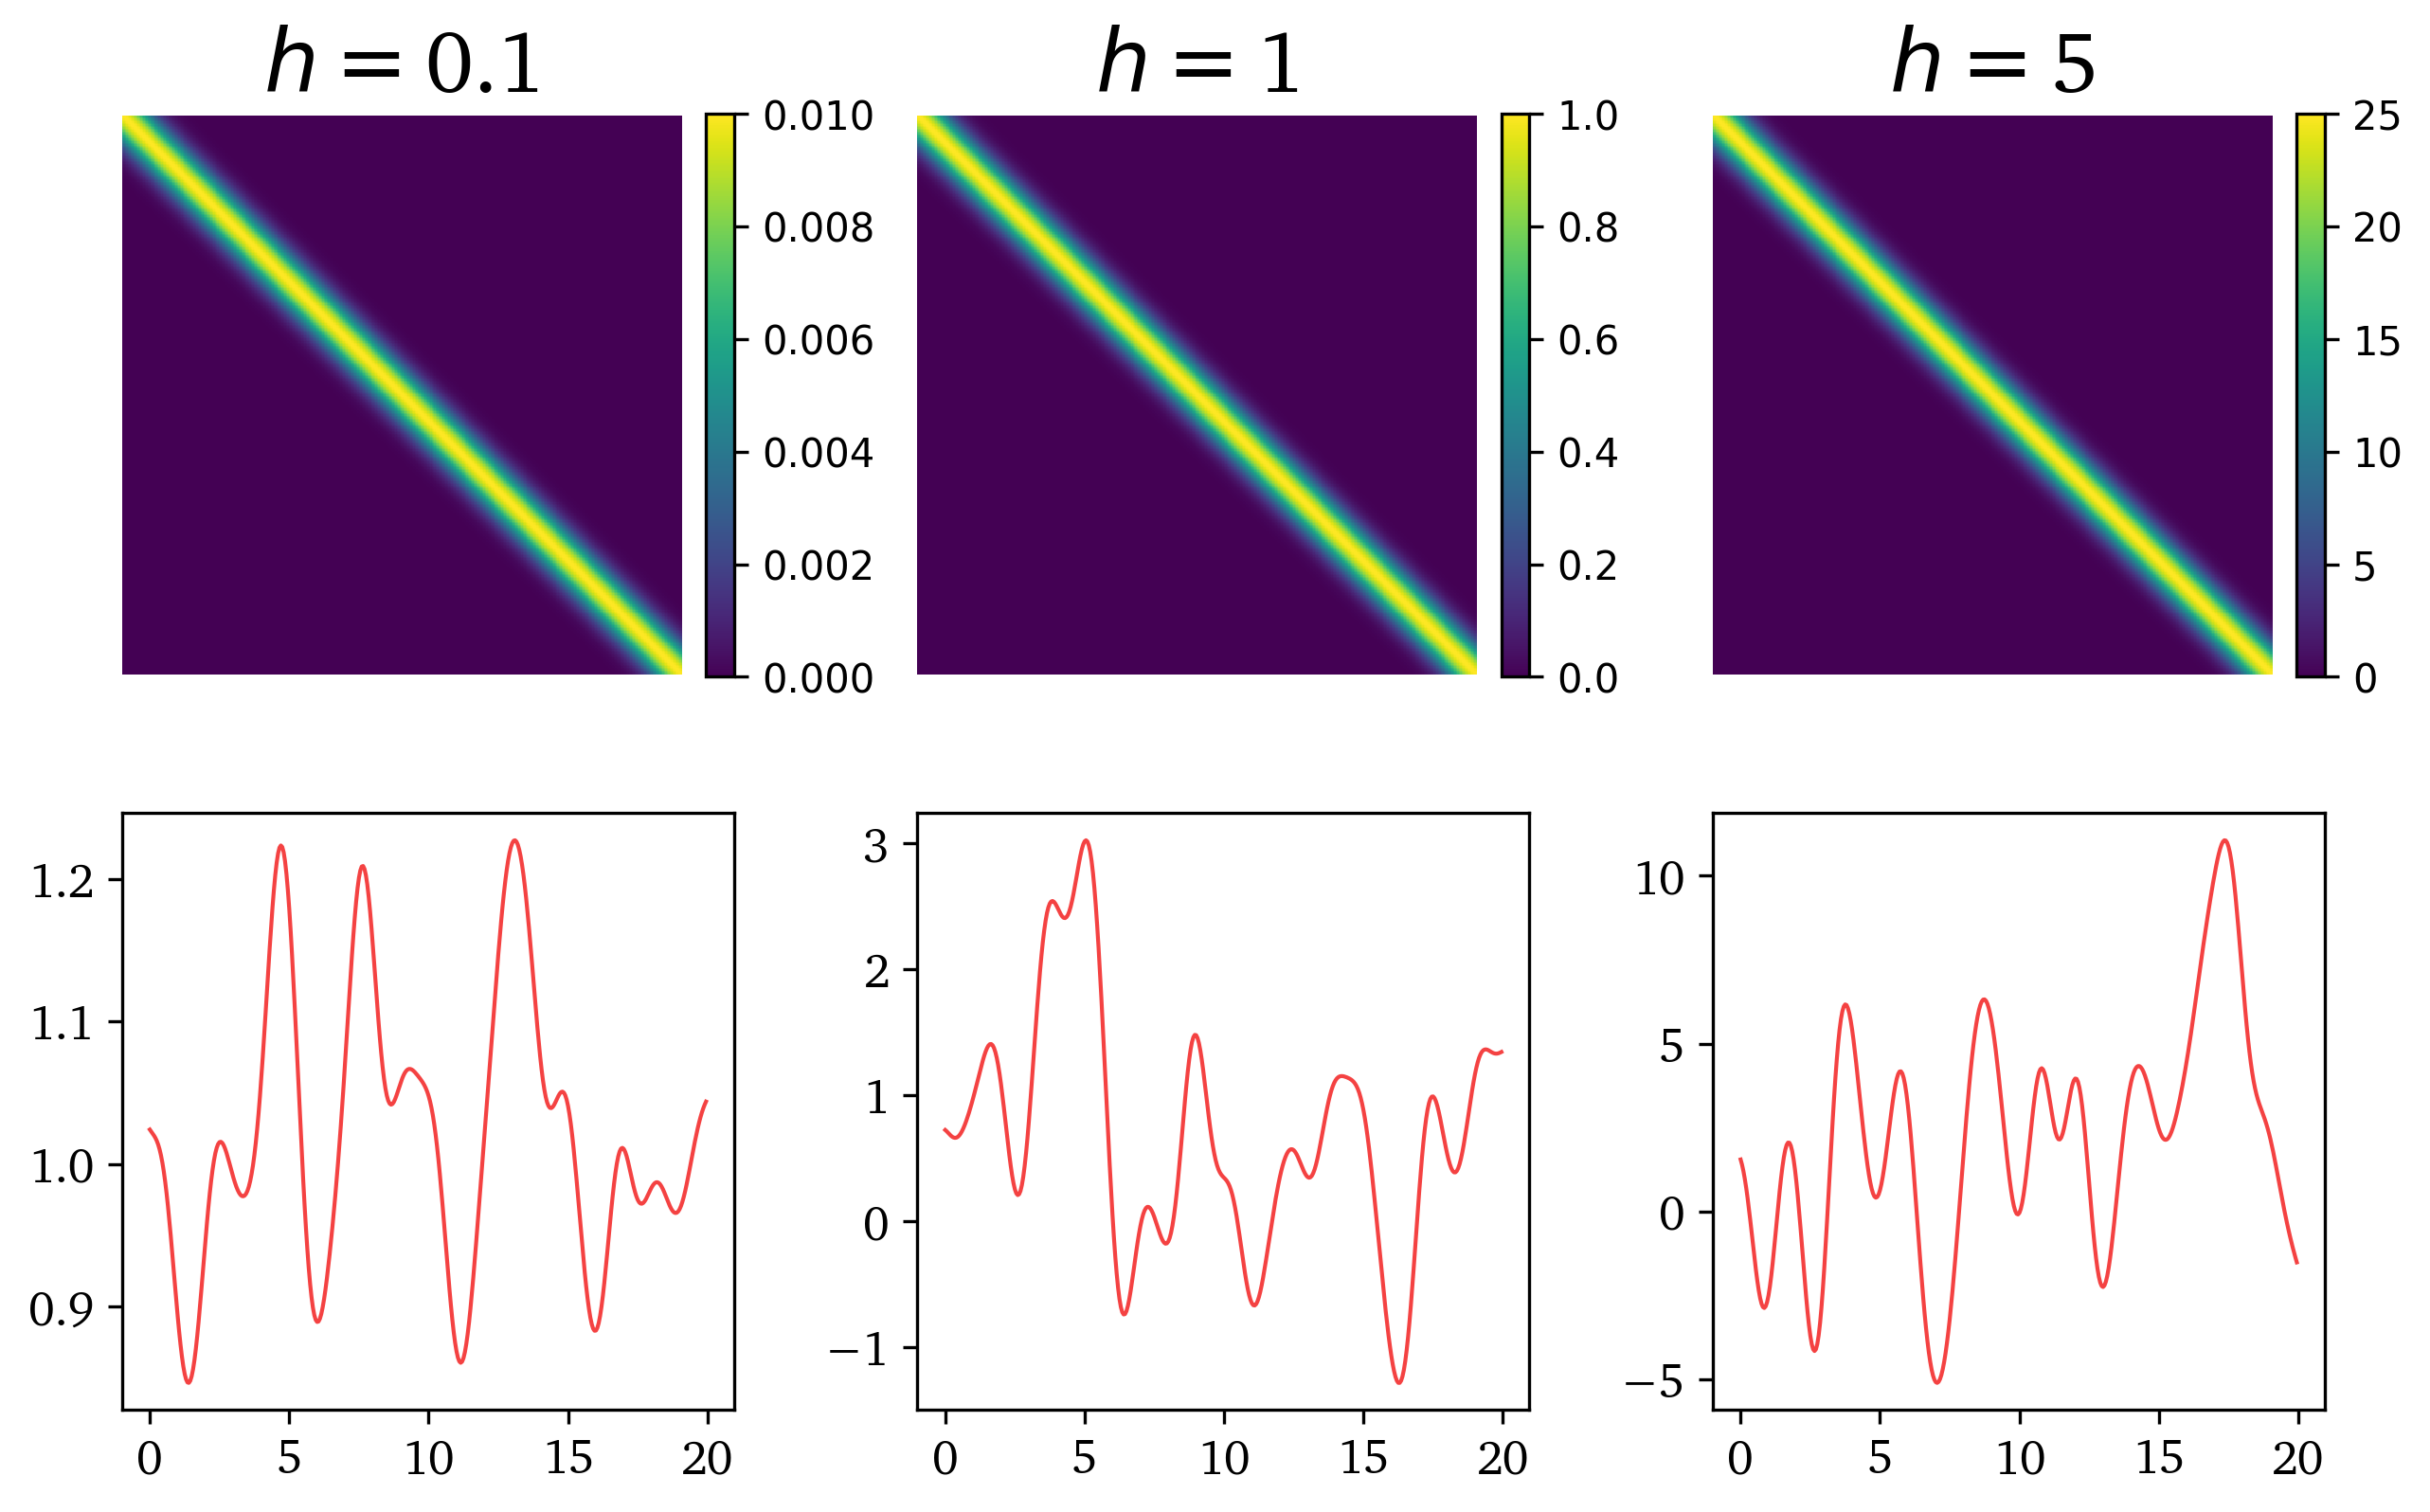
\includegraphics[width=8.5cm]{cov-Kernel-SE-changing-h-tex.png}
\caption{Adjusting the kernel scaling factor $h$.}
\label{fig:SE-kernel-scaling-factor}
\end{figure}

\subsection{What is Gaussian in a Gaussian Process?}

The mean value of the distribution is reflected in the $y$-axis values in Fig. \ref{fig:SE-kernel-width} and \ref{fig:SE-kernel-scaling-factor}. It is yet more evident to look at the histograms from more than one prior realisation. In Fig. \ref{fig:realisation-histogram} 20 realisations have been drawn and it already becomes visible that the $y$-value distribution starts to have the bell shape with the prescribed mean.


\begin{figure}[H]
\centering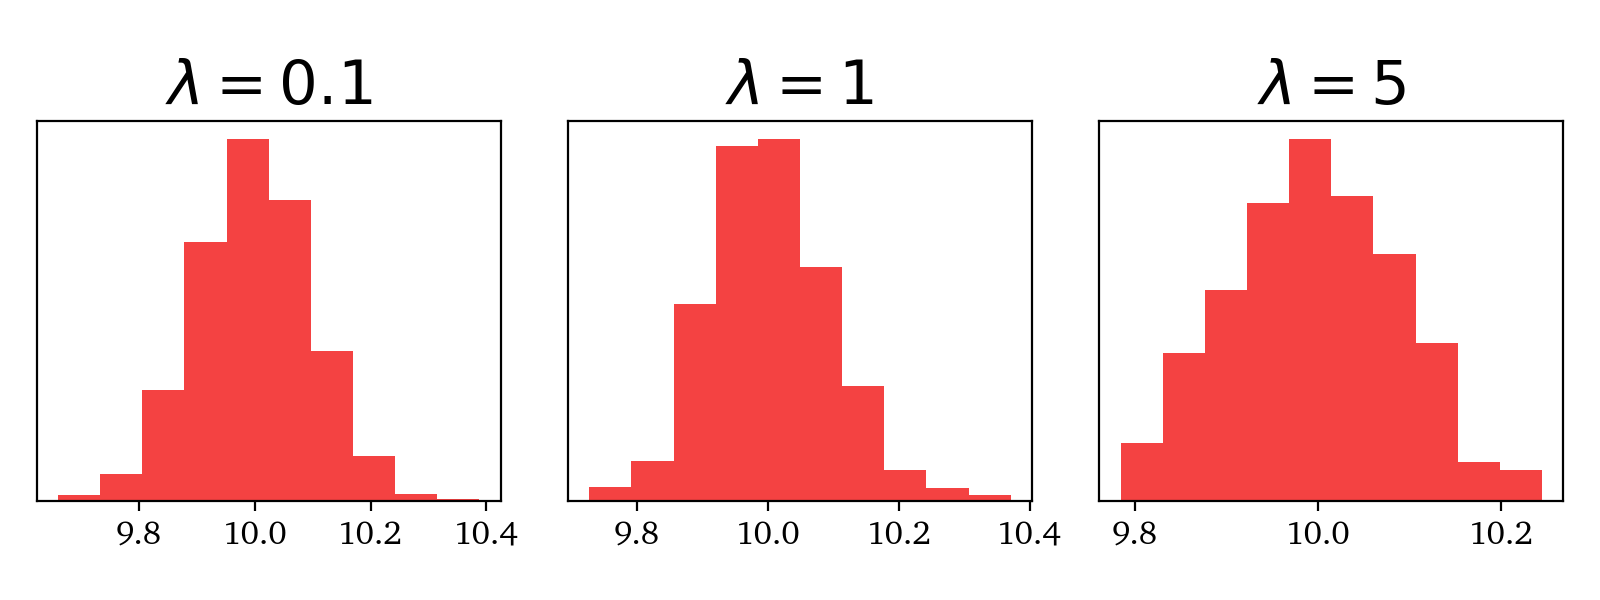
\includegraphics[width=8.5cm]{realisation-Histogram-tex.png}
\caption{Histogram of 20 realisations with mean = 10.}
\label{fig:realisation-histogram}
\end{figure}


This brings us to another interesting point which I so far was hiding from view - the one restriction that is placed on the possible regression functions inside the function pool is that \textbf{all functions have a Gaussian marginal distribution}.
%(Though it does not need to be a case either - GPML uses other likelihoods - but we still call the technique \textbf{Gaussian} Process Regression).
In other words, the histogram of realisations begin to look like a normal distribution as the number of realisations increase.




%\section{Building your GPR in Python}











\thebibliography{}

\bibitem{Rasmussen} C. E. Rasmussen, C. Williams, \textit{Gaussian Process for Machine Learning}, 2006

\bibitem{GP_for_TM} S. Roberts, M. Osborne, M. Ebden, S. Reece, N. Gibson, S. Aigrain \textit{Gaussian Processes for Timeseries Modelling}, 2012

\bibitem{Scaife} A. Scaife, \textit{Machine Learning: Gaussian Process Modelling in Python}, an online lecture, https://youtu.be/UpsV1y6wMQ8

\bibitem{Foreman-Mackey} D. Foreman-Mackey, \textit{Time Series Analysis Using Gaussian Processes in Python \& the Search for Earth 2.0}, an online lecture, https://youtu.be/WhoFbu9dBe0

\bibitem{Malik} M. R. Malik, B. J. Isaac, A. Coussement, P. J. Smith, A. Parente, \textit{Principal component analysis coupled with nonlinear regression for chemistry reduction}, Combustion and Flame 187 (2018) 30-41

\bibitem{SE} https://stats.stackexchange.com/questions/376141/what-is-a-distribution-over-functions

\bibitem{} https://matthewdharris.com/2016/05/16/gaussian-process-hyperparameter-estimation/

\bibitem{kernel-cookbook} D. Duvenaud, \textit{The Kernel Cookbook: Advice on Covariance functions}, https://www.cs.toronto.edu/~duvenaud/cookbook/


\bibitem{duvenaud-thesis} D. Duvenaud, \textit{Automatic Model Construction with Gaussian Processes}, PhD thesis,  University of Cambridge, 2014

\bibitem{George} S. Ambikasaran, D. Foreman-Mackey, L. Greengard, D. W. Hogg, M. O'Neil, \textit{Fast Direct Methods for Gaussian Processes}, 2014



\end{document}
